% The complement of a union is the intersection of the complements.
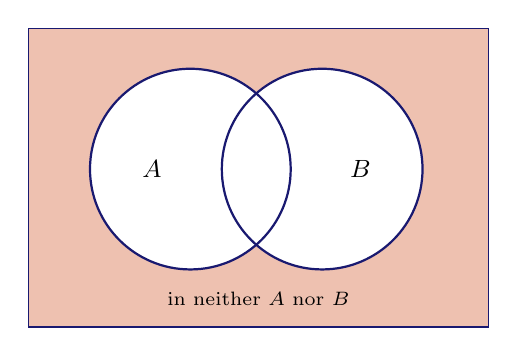
\begin{tikzpicture}[line cap=round,scale=1.08]
  \draw[MidnightBlue,thick] (0,0) rectangle (5.4,3.5);
  \node[font=\small,anchor=north west,text=black] at (0.08,3.42) {$U$};
  \begin{scope}
    \clip (0,0) rectangle (5.4,3.5);
    \fill[BrickRed!22] (0,0) rectangle (5.4,3.5);
    \fill[white] (1.9,1.85) circle (1.18);
    \fill[white] (3.45,1.85) circle (1.18);
  \end{scope}
  \draw[MidnightBlue,thick] (1.9,1.85) circle (1.18);
  \draw[MidnightBlue,thick] (3.45,1.85) circle (1.18);
  \node[font=\small] at (1.45,1.85) {$A$};
  \node[font=\small] at (3.9,1.85) {$B$};
  \node[font=\scriptsize,align=center,text=black] at (2.7,0.32) {in neither $A$ nor $B$};
\end{tikzpicture}
